% !TeX root = thesis.tex
\documentclass{master_thesis}
\addbibresource{refs.bib}

\begin{document}

\section{Results} \label{chap:results}

% The nucleus of your dissertation, the results chapter thoroughly explores your findings. This is where you present your data or original analysis, along with any visual aids, such as graphs or charts.

% For empirical dissertations, structure the results section by individual data findings, analyzed in depth one by one. For nonempirical dissertations, structure this section by themes, patterns, or trends you’ve noticed in your research.

% Don’t forget to relate your findings back to the central research question or thesis statement.

\subsection{Current state of awareness about accessibility in Pipedrive}

As the first step of the research, a survey was shared in Pipedive's Slack channels (Figure \ref{fig:slack-message}) to understand what is the knowledge and general approach to web accessibility in the company. It was shared in 4 channels to reach people who are most likely to be dealing with accessibility, the component library and who are interested in accessibility (Table \ref{table:survey-shared}).

\begin{figure}[ht]
	\centering
	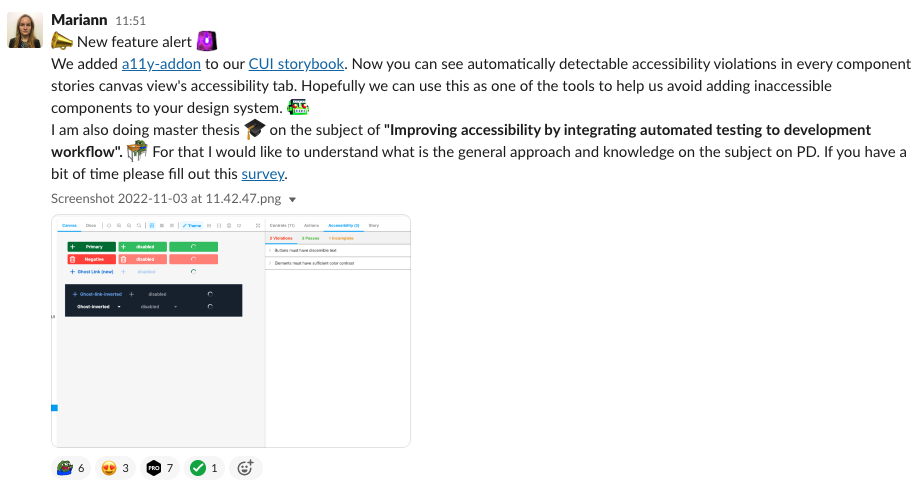
\includegraphics[width=\textwidth]{img/survey.png}
	\caption[Message in company Slack about accessibility tool and survey.]{Message in company Slack announcing adding accessibility tool and inviting people to reply to the survey.}
	\label{fig:slack-message}
\end{figure}

\begin{table}[H]
	\centering
	\begin{tabular}{|l|l|}
		\hline
		\textbf{Channel members or theme} & \textbf{number of members}  \\
		\hline
		Front end developers  & 212  \\
		\hline
		Dedicated to our component library  & 124  \\
		\hline
		Designers  & 73  \\
		\hline
		Accessibility channel  & 31  \\
		\hline
	\end{tabular}
	\caption{List of all the channels the survey was shared in.}
	\label{table:survey-shared}
\end{table}

Some people might also be on more than one of these channels. The aim was to reach people in the company who would be most likely to be using these tools and contribute to the library. There were 7 questions and some of them also included a field for free text to give more details on the subject if they wanted (Appendix \ref{appendix:pre-survey-questions}).

In total, 20 people replied to the survey - 6 designers and 14 developers, including one engineering manager. This does not give a full overview of the company, but it should give a good insight into the general opinions regarding accessibility. Likely, developers and designers that are more involved with our component library and/or are interested in accessibility were more likely to respond.

\textbf{RQ1:} "How good is the knowledge about accessibility standards, tools and best practices in the company before integrating the accessibility testing tool?" is answered by the results of this survey. They show that 10\% of people who responded think their knowledge of accessibility is very good, while most think that their knowledge level is average and none of the responders judge their knowledge about accessibility to be very good (Figure \ref{fig:a11y-knowledge-current}). 35\% of people who participated in the survey know where to find resources about accessibility standards, 15\% don't know and 50\% know, but think they need more (Figure \ref{fig:a11y-resources}).

\begin{figure}[ht]
    \centering
	\begin{subfigure}{0.5\textwidth}
		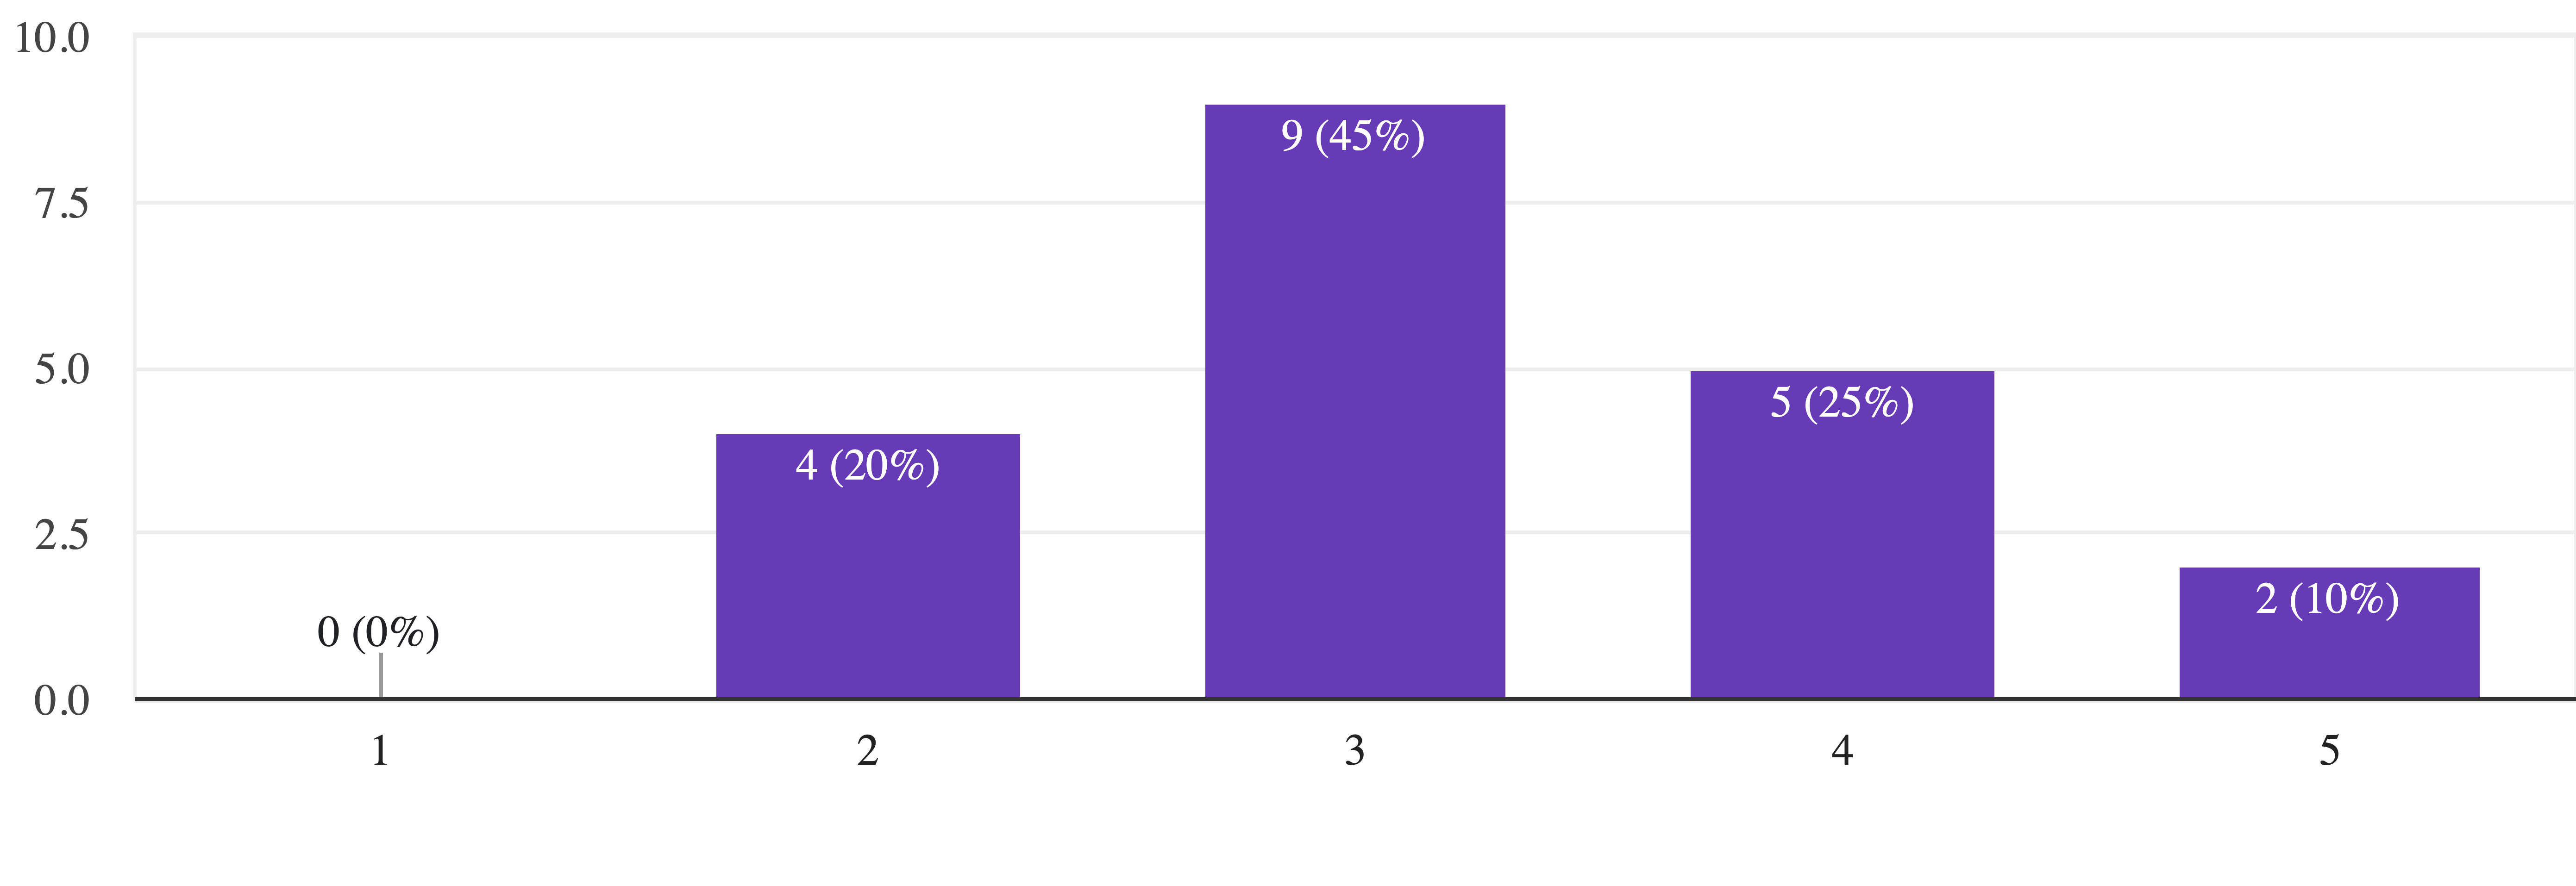
\includegraphics[width=\textwidth]{img/a11y-knowledge.png}
		\caption{Pre-case study survey: How much do you know about accessibility (standards, best practices, importance, testing)? 1- "Almost no knowledge" to 5 - "I have very good knowledge" }
		\label{fig:a11y-knowledge-current}
	\end{subfigure}
	\hspace{0.05\textwidth}
	\begin{subfigure}{0.4\textwidth}
		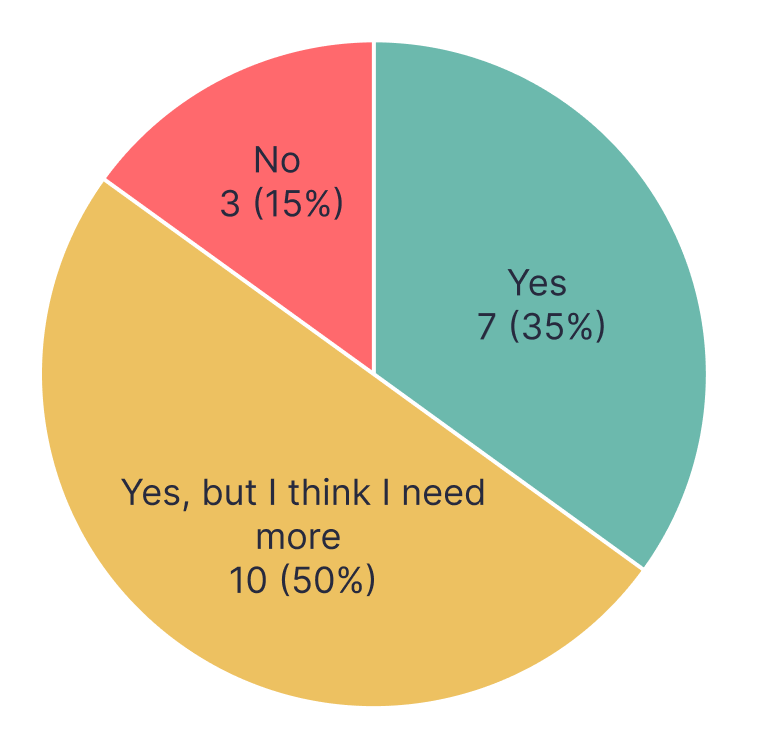
\includegraphics[width=\textwidth]{img/a11y-resources.png}
		\caption{Do you know where to find resources
		about accessibility standards? (no one chose the 4th option "No I don't think I need them") }
    	\label{fig:a11y-resources}
	\end{subfigure}
	\caption{Accessibility knowledge in Pipedrive}
    \label{fig:a11y-knowledge}
\end{figure}

Most people who replied to the survey don't think accessibility is being prioritized in Pipedrive and at the same time, most of them think that Pipedrive should be putting more focus on following common accessibility standards (Figure \ref{fig:a11y-priority}). They elaborated on what they think are the reasons behind this in the free text answers to questions 4 and 6.

Based on the replies received, accessibility has always been seen as something that is low on Pipedrive's list of priorities and there has not been any clear company-wide strategy on how to manage and improve it. There has never been a dedicated project manager to bring focus to this subject and right now developers and designers are the ones that seem to be responsible for it.
Two people think that it would not affect Pipedrive's customers much. All replies can be seen in  Appendix \ref{appendix:post-survey-responses}.

\begin{figure}[ht]
    \centering
	\begin{subfigure}{0.45\textwidth}
		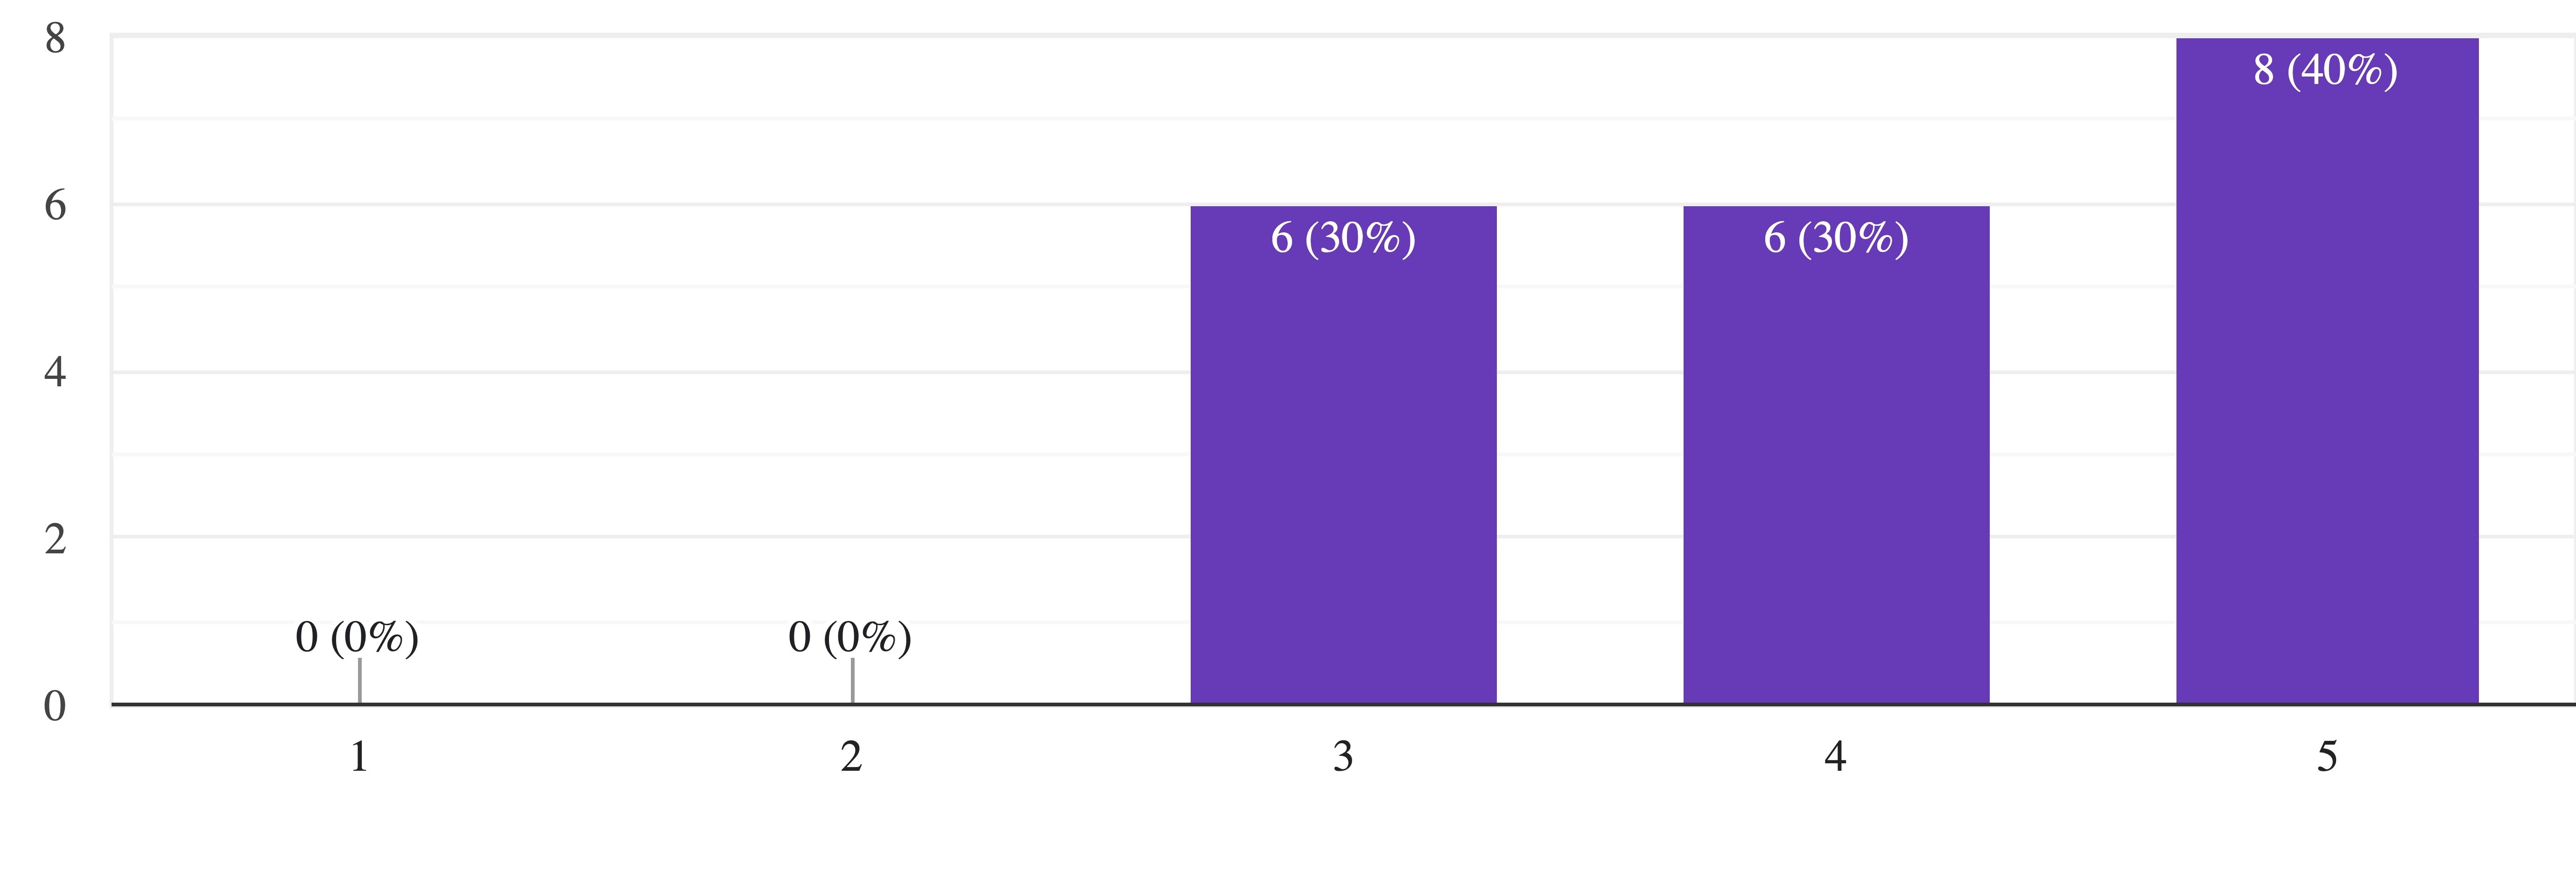
\includegraphics[width=\textwidth]{img/a11y-priority.png}
		\caption{Do you think accessibility is a priority in our company? 1-No not at all to 5-Yes very much \\
		\\
		\\}
	\end{subfigure}
	\hspace{0.05\textwidth}
	\begin{subfigure}{0.45\textwidth}
		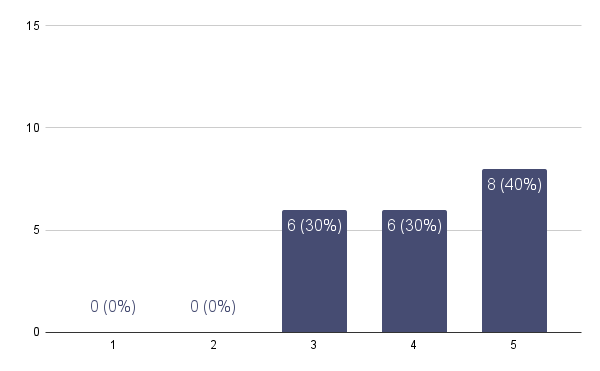
\includegraphics[width=\textwidth]{img/a11y-goals.png}
		\caption{Do you think we should prioritize following accessibility standards (like \ac{wcag}, EN 301 549) in our product? 1- "No I think they are irrelevant for Pipedrive customers" to 5 - "Yes I think following accessibility standards should be a high priority" }
	\end{subfigure}
	\caption{Priority of accessibility in Pipedrive}
    \label{fig:a11y-priority}
\end{figure}

It seems like with most things more knowledge about the business impact of accessibility would help prioritize solving these problems. There is a lot currently that could be improved, but it could be argued that implementing a way of continuously testing for at least some accessibility issues from the beginning of all new developments could help to ensure that the technical debt related to accessibility would not grow to be even bigger. There were several comments in the free text sections expressing that they appreciate this subject being brought to focus and even some offering to help.

\subsection{Results from Manual Audit and Automated Tests}

A summary table was created from all violations and passes found while running the automated accessibility tests and all the violations found in the manual audit. The listed violations and passes were counted to obtain numerical data that can be analyzed using statistical methods (Appendix \ref{appendix:results-table}).

% summary of violations
The results show that addon-a11y did not report any violations for 27 (51\%) components out of 53 components. After verifying, the validity of these issues the number goes up to 31 (58\%). On average, the automated testing tool found 1 violation per component. The maximum number of violations reported for a single component was 7 and the maximum number of valid violations was 6 (Figure \ref{fig:audit-combined}).

\begin{figure}[H]
	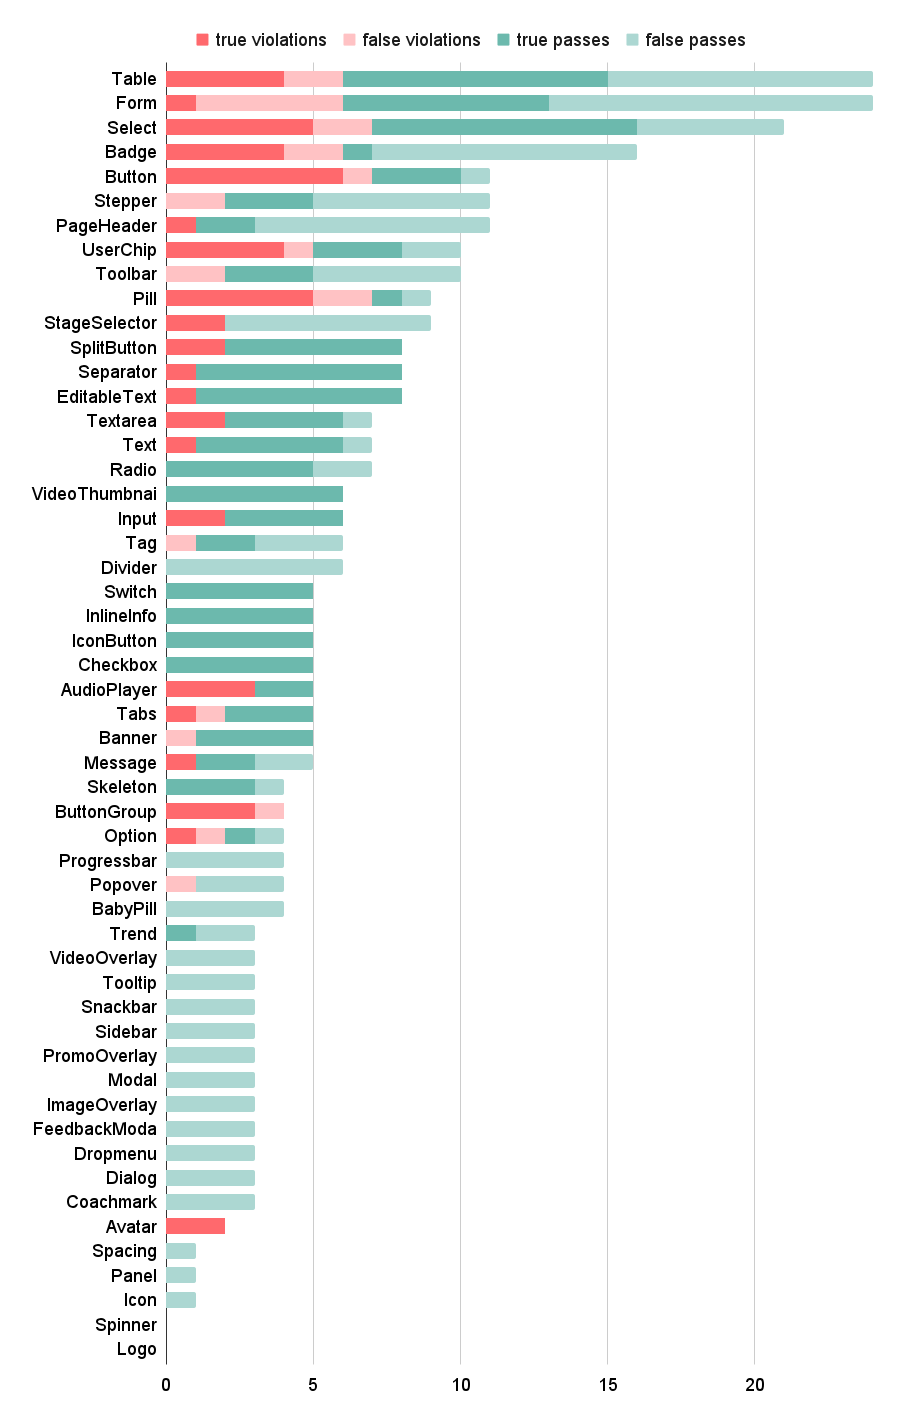
\includegraphics[width=\textwidth]{img/audit-combined.png}
	\caption{Violations and passes detected by addon-a11y}
	\label{fig:audit-combined}
\end{figure}

% summary of passes
Four components out of 53 did not have any passed checks and 22 did not have any valid passed checks (see figure \ref{fig:audit-combined}). This means that the number of components with no valid passed checks changed from 4\%  to 42\% after manually validating the results. The highest number of passes - 18 - was detected in \textit{Form} and \textit{Table} components. After validating, the number of passes changed to 9 for \textit{Table} and 7 for \textit{Form}. The average number of passes for each component was 5, which decreased to 2 after validating the results.

\begin{figure}[ht]
	\begin{subfigure}{0.45\textwidth}
	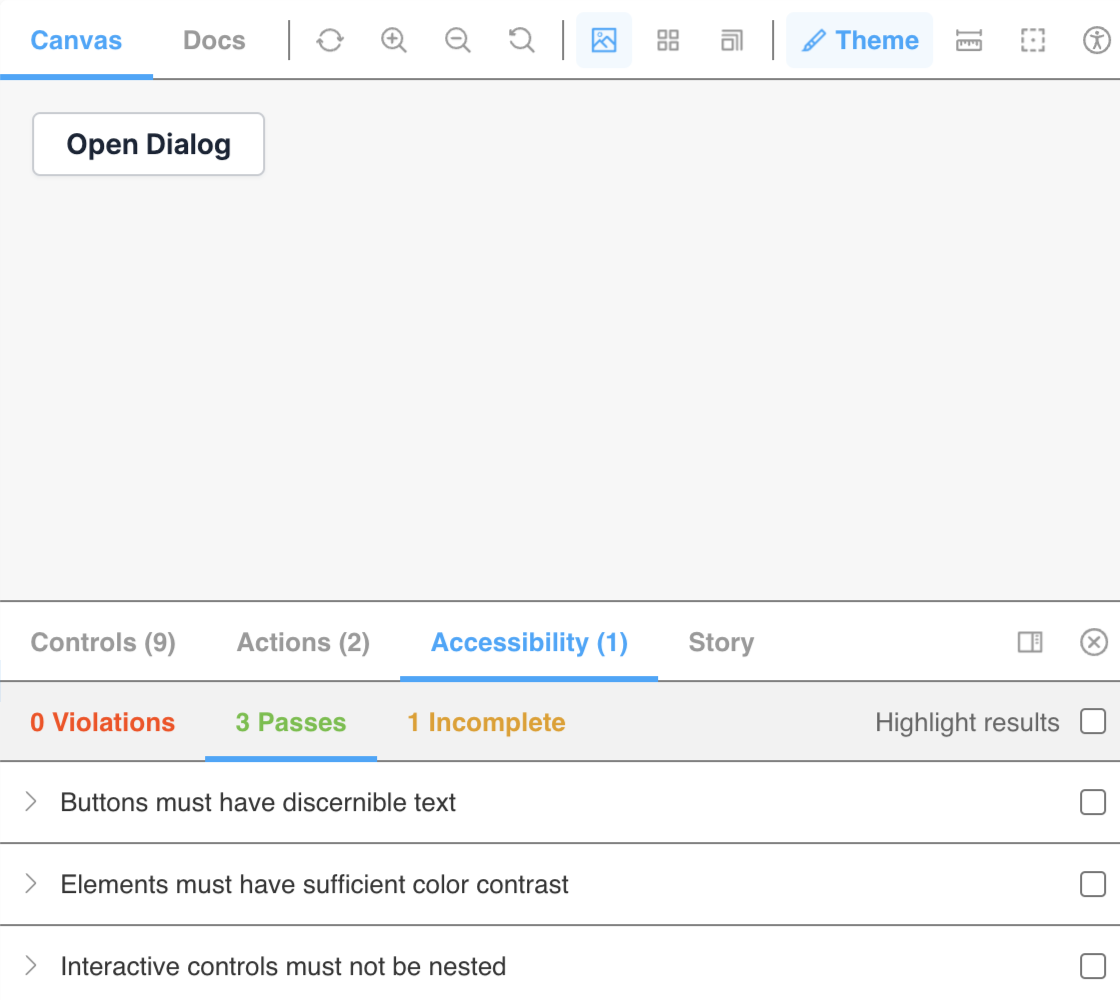
\includegraphics[width=\textwidth]{img/sb-button-trigger.png}
	\caption{Inital view of example. This is tested by addon-a11y.}
	\label{fig:sb-button-trigger-1}
	\end{subfigure}
	\hspace{0.05\textwidth}
	\begin{subfigure}{0.45\textwidth}
	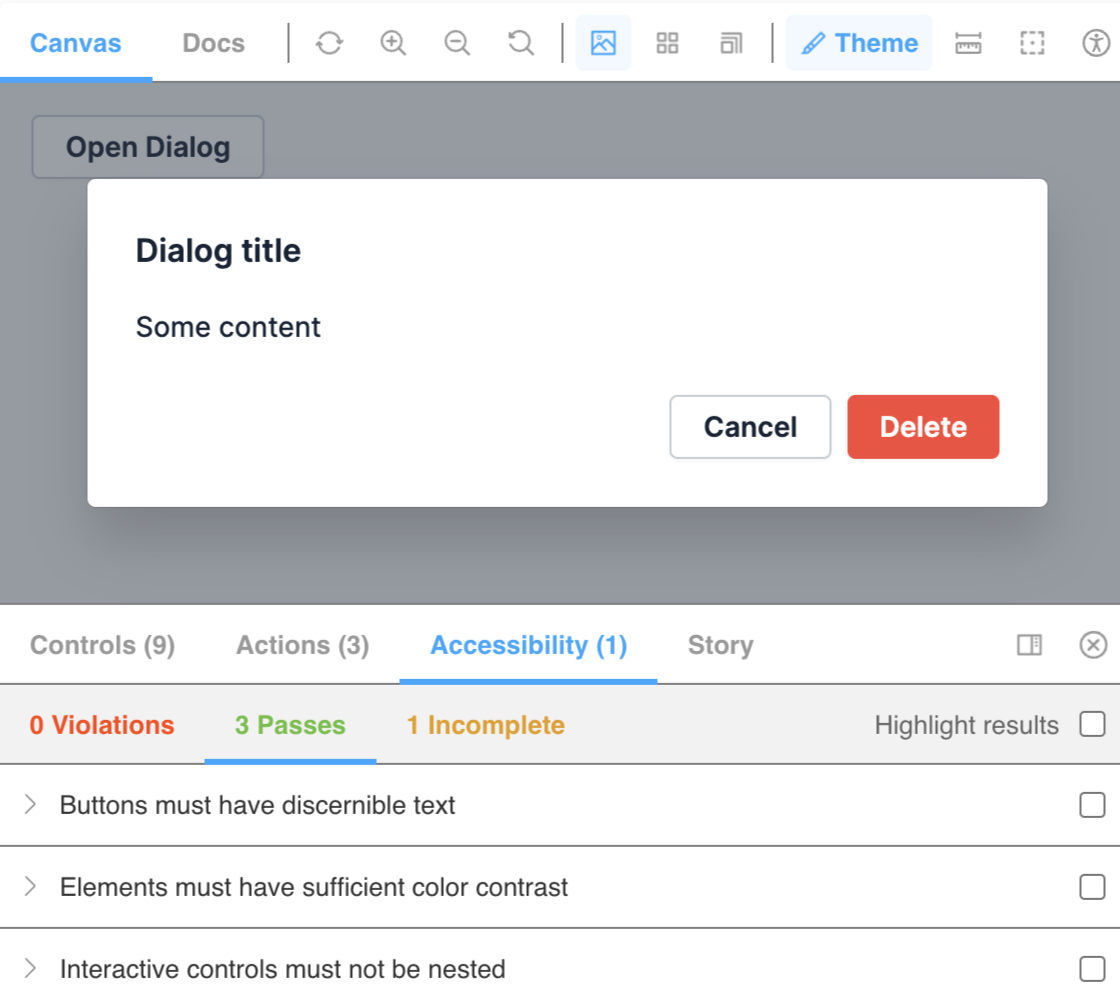
\includegraphics[width=\textwidth]{img/sb-button-trigger-open.png}
	\caption{Example after clicking the button and revealing the actual component.}
	\label{fig:sb-button-trigger-2}
	\end{subfigure}
\caption{Storybook example for Dialog component using a button trigger}
\label{fig:sb-button-trigger}
\end{figure}



% \begin{figure}[H]
% 	\centering
% 	\begin{subfigure}{0.24\textwidth}
% 	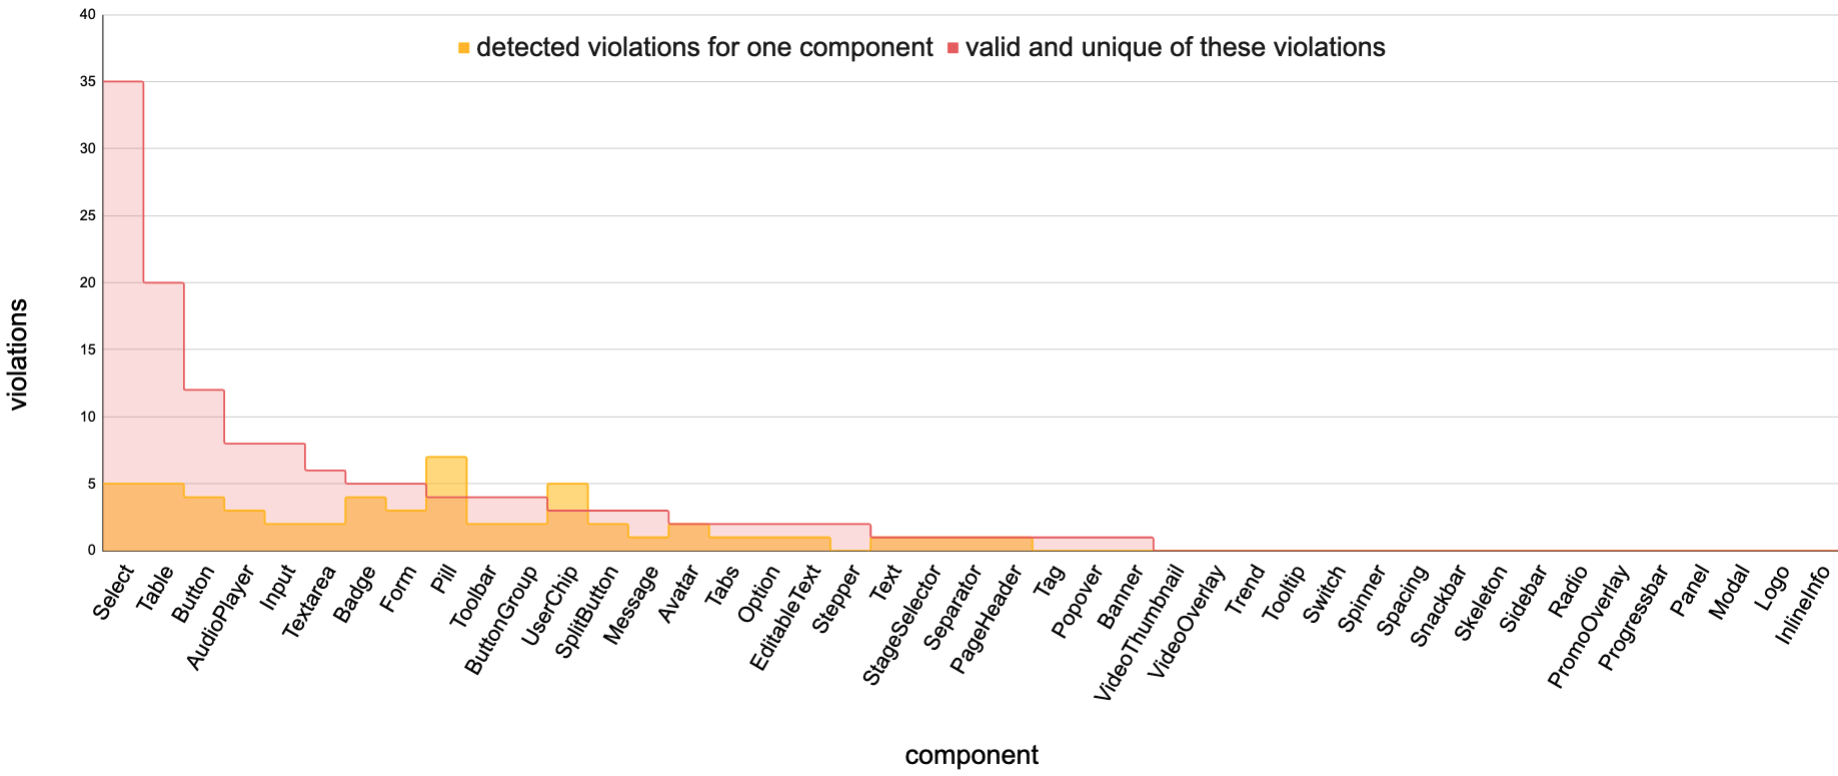
\includegraphics[height=0.7\textheight]{img/audit-failed.png}
% 	\caption{All violations reported by addon-a11y and how many of them are valid.}
% 	\label{fig:audit-failed}
% 	\end{subfigure}
% 	% \hspace{0.05\textwidth}
% 	\begin{subfigure}{0.34\textwidth}
% 	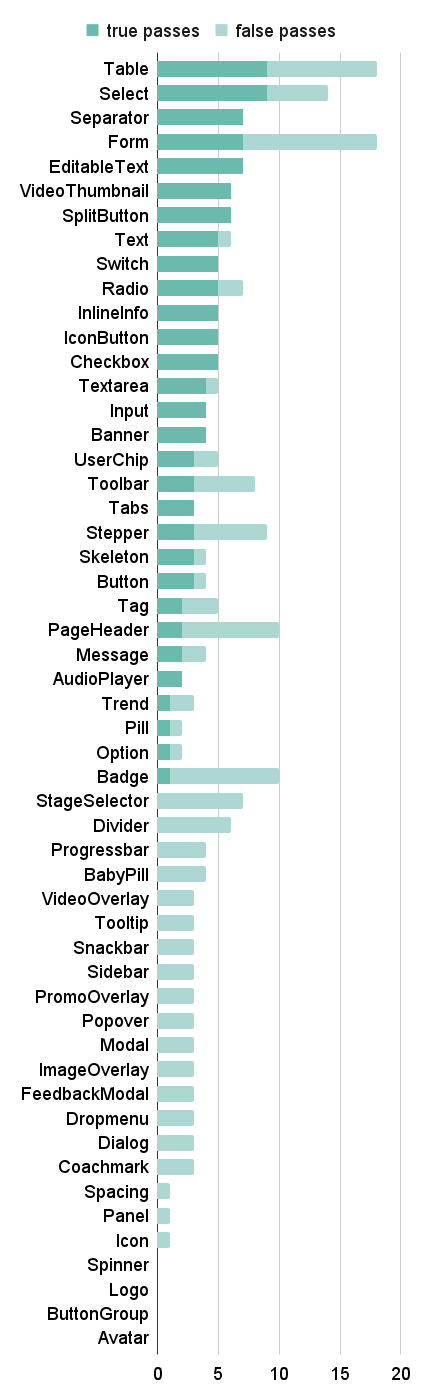
\includegraphics[height=0.7\textheight]{img/audit-passed.png}
% 	\caption{All passed checks reported by addon-a11y and how many of them are valid.}
% 	\label{fig:audit-passed}
% 	\end{subfigure}
% 	\begin{subfigure}{0.39\textwidth}
% 	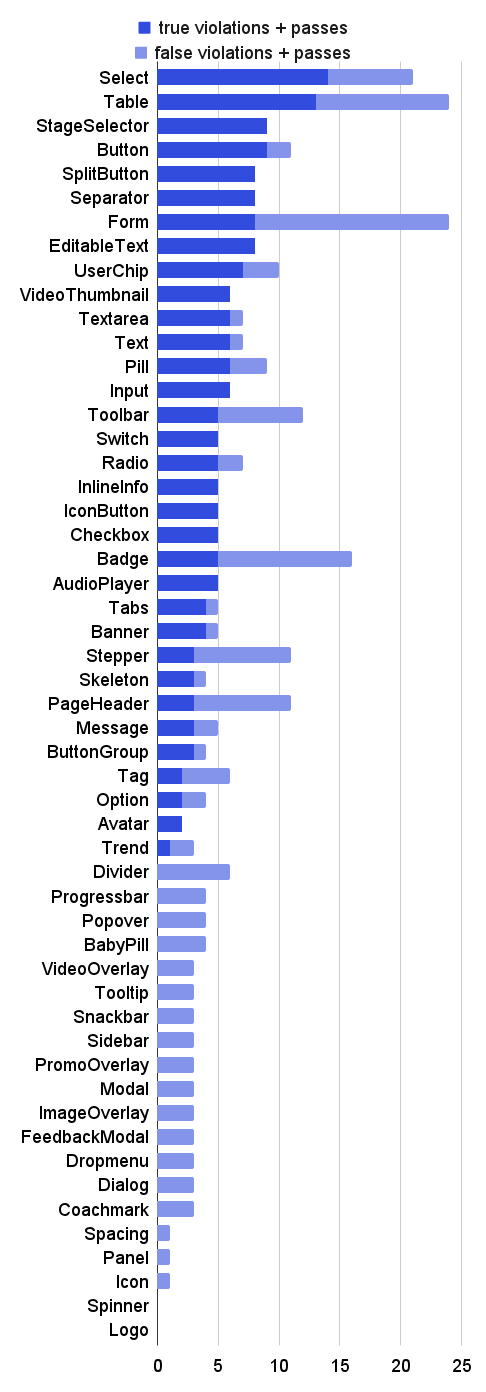
\includegraphics[height=0.7\textheight]{img/audit-all.png}
% 	\caption{All checks performed by addon-a11y and how many of them are valid.}
% 	\label{fig:audit-all}
% 	\end{subfigure}
% \caption{All issues checked by addon-a11y}
% \label{fig:audit-passed-failed}
% \end{figure}


% summary of violations + passes
Looking at all the fails and passes gave a good overview of how many tests were run for each component. Out of 53 components that were tested, only 2 (4\%) did not get checked by addon-a11y at all, but some of the ones that did get tested included false violations or passes. After validating the results, the number of components that were not tested increased to 20 (38\%). This number includes components that become visible only when triggered by another element, like modals and popups for which the examples in Storybook only displayed a trigger button (Figure \ref{fig:sb-button-trigger}). In total, there were 11 components with examples like that and they can be seen in Figure \ref{fig:audit-combined} starting from \textit{VideoOverlay} and ending with \textit{Coachmark}.

The components that are displayed with a trigger button would normally open when triggered by something, and the examples are intended to resemble how they would be used in real life. Brick-ui was used to explore different ways of mitigating this. Testing revealed that these kinds of examples could be improved in Storybook 7 by adding a user interaction that opens the component. Accessibility tests are run after this mocked user interaction has been executed. In Storybook 6 the same thing could be achieved by opening the example manually and triggering a rerun of the accessibility checks. It is important to make sure that the opened component is rendered inside the div element with id="root" (or "storybook-root" in version 7). All 11 components were retested in Storybook with addon-a11y with the changes described above made. Accessibility checks could only be triggered in one of the examples of \textit{Tooltip} and on of the examples of \textit{Modal}. The rest of the components need more improvements to their examples. It is possible to render all the components except \textit{VideoOverlay} and \textit{FeedbackModal} inside the root element. This means that with improved examples, tests could be run for these components. At the time of the case study, there was a bug in axe-core that caused most of the components to be ignored even if all the requirements described above were fulfilled.

The remainder of the components that did not get tested by the addon included very simple components for spacing and visuals. These need further testing when they are being used in context to make sure that the visual info they are conveying is also included in text form. The results from manual testing did not reveal any additional issues for 6 of the components that did not get tested. Manual testing revealed the most additional issues for the components that have a trigger button in the examples. This is expected as due to the limitation of the examples the correct component was not evaluated by the tool.

Analyzing the validity of checks performed by addon-a11y further shows that from all the passes and violations together, a bit more than half were valid while 68\% of the detected violations were correct and 51\% of passed checks were confirmed to be relevant (Figure \ref{fig:checks-validity}).

\begin{figure}[ht]
	\centering
	\begin{subfigure}{0.3\textwidth}
	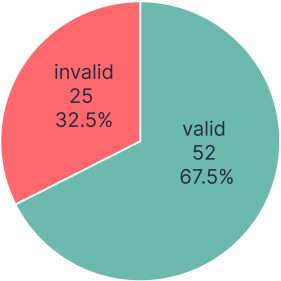
\includegraphics[width=\textwidth]{img/violations.png}
	\caption{How many of the detected violations are valid?}
	\label{fig:checks-validity-failed}
	\end{subfigure}
	\hspace{0.03\textwidth}
	\begin{subfigure}{0.3\textwidth}
	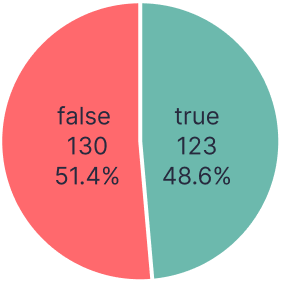
\includegraphics[width=\textwidth]{img/passes.png}
	\caption{How many of the passes are valid?}
	\label{fig:checks-validity-passed}
	\end{subfigure}
	\hspace{0.03\textwidth}
	\begin{subfigure}{0.3\textwidth}
	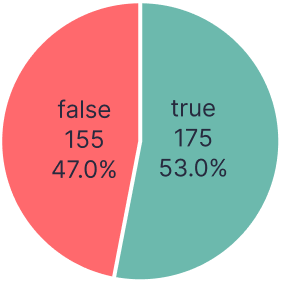
\includegraphics[width=\textwidth]{img/violations+passes.png}
	\caption{How many of all violations and tests combined are valid?}
	\label{fig:checks-validity-all}
	\end{subfigure}
\caption{Validity of tests performed by addon-a11y}
\label{fig:checks-validity}
\end{figure}

\textbf{RQ2}: "What kind of errors can be caught by running automated accessibility tests on a component library?" can be answered based on these results and the results from manually evaluating the same components. The \ac{wcag} Success Criterion that proved to be reliably testable in Pipedrive's component library are:

\begin{itemize}
	\item Success Criterion 1.1.1 Non-text Content
	% (https://www.w3.org/TR/WCAG21/#non-text-content)
	% \begin{itemize}
	% 	\item Images must have alternate text
	% \end{itemize}

	\item Success Criterion 1.3.1 Info and Relationships
	% https://www.w3.org/TR/WCAG21/#info-and-relationships
	% \begin{itemize}
	% 	\item Certain ARIA roles must contain particular children
	% \end{itemize}

	\item Success Criterion 1.4.3 Contrast (Minimum)
	% (https://www.w3.org/TR/WCAG21/\#contrast-minimum)
	\item Success Criterion 1.4.6 Contrast (Enhanced)
	% (https://www.w3.org/TR/WCAG21/\#contrast-enhanced)
	% \begin{itemize}
	% 	\item Color contrast
	% \end{itemize}

	\item Success Criterion 1.4.12 Text Spacing
	% (https://www.w3.org/TR/WCAG21/#text-spacing)
	% \begin{itemize}
	% 	\item Inline text spacing must be adjustable with custom stylesheets
	% \end{itemize}

	\item Success Criterion 2.1.1 Keyboard
	\item Success Criterion 2.1.3 Keyboard (No Exception)
	% (https://www.w3.org/TR/WCAG21/#keyboard)
	% (https://www.w3.org/TR/WCAG21/#keyboard-no-exception)
	% \begin{itemize}
	% 	\item Scrollable region must have keyboard access
	% \end{itemize}

	\item Success Criterion 2.4.4 Link Purpose (In Context)
	\item Success Criterion 2.4.9 Link Purpose (Link Only)
	% (https://www.w3.org/TR/WCAG21/#link-purpose-in-context)
	% (https://www.w3.org/TR/WCAG21/#link-purpose-link-only)
	% \begin{itemize}
	% 	\item Links with the same name must have a similar purpose
	% 	\item Links must have discernible text
	% \end{itemize}

	\item Success Criterion 4.1.1 Parsing
	% (https://www.w3.org/TR/WCAG21/#parsing)
	% \begin{itemize}
	% 	\item IDs used in ARIA and labels must be unique
	% \end{itemize}

	\item Success Criterion 4.1.2 Name, Role, Value
	% (https://www.w3.org/TR/WCAG21/\#name-role-value)
	% \begin{itemize}
	% 	\item Buttons must have discernible text
	% 	\item Form elements must have labels
	% 	\item Form field must not have multiple label elements
	% 	\item Form elements should have a visible label
	% 	\item ARIA input fields must have an accessible name
	% 	\item ARIA roles used must conform to valid values
	% 	\item ARIA commands must have an accessible name
	% 	\item Interactive controls must not be nested
	% \end{itemize}

	% \item Correct usage of WAI-ARIA
	% (https://www.w3.org/TR/wai-aria-1.1/#usage)
	% \begin{itemize}
	% 	\item ARIA attributes must conform to valid values
	% 	\item ARIA attributes must conform to valid names
	% 	\item Elements must only use allowed ARIA attributes
	% 	\item Required ARIA attributes must be provided
	% \end{itemize}

	% \item Best Practices Rules
	% \begin{itemize}
	% 	\item ARIA role should be appropriate for the element
	% 	\item Elements should not have tab index greater than zero
	% 	\item Alternative text of images should not be repeated as text
	% 	\item Headings should not be empty
	% 	\item Heading levels should only increase by one
	% \end{itemize}
\end{itemize}

In addition to these, axe-core automated accessibility testing engine tested for the correct usage of \ac{wai-aria} and best practices that are defined by the developers of the testing tool based on the accepted practices in the industry. Deque's Github repository lists a total of 87 testable accessibility rules that are enabled by default in axe-core \citep{Fiers2023}. Of those, 58 check for conformance with \ac{wcag} 2.0 and 2.1 level A and AA success criteria and 29 are best practices that can't necessarily be mapped to \ac{wcag} but should indicate industry-accepted practices for improvements that can be made to the overall user experience. This shows that axe-core testing engine is capable of testing more than what was listed above, but these issues might just not have been represented in Pipedrive's components and examples.

The most commonly valid test result was color contrast with 45,1\% of all violations and passes being color contrast issues. It is also important to note that axe-core can reliably test for the existence of the alt attribute in an image, but it is not capable of judging how accurate or informative the content of the alt attribute is or even whether the image is purely decorative and should have an empty alt value.

Based on the additional issues found in the manual audit, it could be concluded that the following issues should be manually tested:
\begin{itemize}
	\item Focus states
	\item Navigating and interacting using a keyboard
	\item Navigating and interacting using a screen reader
	% \item Recognizable color differences between semantically different variants of one component
	\item Images and what should be the values of their alt texts
	\item \ac{svg}s and if they should have an aria-label (text alternative) and if so, what should it be
\end{itemize}

Evaluating the accessibility of focus states with automated testing could potentially be improved by using pseudo states add-on and writing better examples for components that would also display it in all relevant focus states.

% What could be improved in component examples to make them more testable
Inaccurate results and missed issues indicated problems with how the component examples had been written. The following things could be improved to get better results from automated testing:
\begin{itemize}
	\item Variants of components that are meant to be used on dark backgrounds should always be displayed on a dark background
	\item Examples where the component gets triggered by a button should be avoided when possible or made visible to the testing tool by other means
	\item Examples should be simple and display one component at a time to reduce the number of tests being run that are irrelevant to the isolated component
	\item Pseudo-classes (like hover, focus etc) of interactive elements should be displayed in the examples
\end{itemize}

\subsection{How Much Was Compliance with WCAG Improved?}

One of the benefits of using automated testing tools is the improved observability of the state of accessibility.
Multiple accessibility reports were generated in Pipedrive's component library during the time when the usage of the automated testing tool was observed. The reports counted different
issues, but for the purpose of this study and for observing the overall accessibility improvement process, the total number of detected violations was compared. (Figure \ref{fig:automted-reports}).

\begin{figure}[ht]
	\centering
	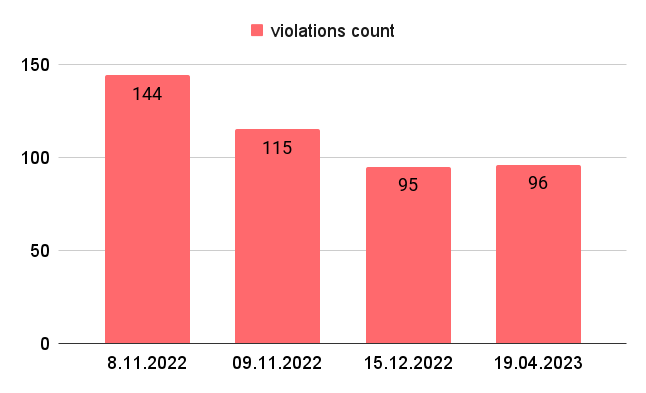
\includegraphics[width=0.8\textwidth]{img/automated-audit-reports.png}
	\caption{How much have automated audit report results improved since adding the tool?}
	\label{fig:automted-reports}
\end{figure}

Results show that over the course of 5 months, the number of accessibility issues was reduced while and immediately after conducting the manual accessibility audit. This is logical because the team involved in performing the audit also had dedicated time to focus on solving these issues. It is also worth noting that several new components were added to the library between the last two reports and the number of accessibility issues did not increase considerably.

As discussed in the previous chapters, automated accessibility testing tools cannot catch all issues. So the fact that almost no additional violations were introduced with the new components alone cannot provide certainty that the component library is just as accessible as it was the last time the report was generated. It could be argued that the biggest value of using automated testing tools in Pipedrive's component library, in addition to finding certain kinds of accessibility violations, has been bringing focus and attention to the subject of accessibility.

\citeauthor{Paterno2020} said that developers find maintaining a high level of accessibility hard because it is only considered after the first release of the product. Having a continuous way to monitor and detect issues should help maintain the level of accessibility that was reached when there was more time to focus on it. The data collected in the short time that this automated accessibility tool has been in use in Pipedrive supports that theory.

A good level of accessibility is easier to achieve when developers consider it from the start of the process. Fixing things in a later phase is more difficult to justify to the business side and is usually more difficult than building an accessible component or webpage from the beginning.

% \info{RQ3: To what extent can integrating automated testing into a component library's development pipeline help improve its compliance with \ac{wcag}? }

Answering \textbf{RQ3}, "To what extent can integrating automated testing into a component library's development pipeline help improve its compliance with WCAG?" is not as simple as examining the reduced number of violations in the automated accessibility testing report. Based on the data gathered in this research, it is not possible to claim conclusively that implementing automated accessibility testing in a component library's development workflow will improve the accessibility of the final product. However, the data does suggest that such integration is highly likely to result in at least some improvement.

The experience of using automated accessibility testing tools and conversations with other developers in the company has suggested that a big benefit of using tools like this is that it makes the whole subject of web accessibility a bit more measurable and less daunting. Having an easy and familiar way of testing for accessibility violations together with links to resources that help solve these issues makes it more likely for developers to take on the task of solving these issues.

\subsection{Limitations of Testing in Component Libraries}

For answering \textbf{RQ4:} "What are the biggest problems of integrating automated accessibility testing into a component library's development workflow?" we should look at the limitations that testing isolated components poses and also more specific issues that were faced during this case study and implementing automated accessibility testing in Storybook with addon-a11y.

Automated accessibility tests are not capable of evaluating all \ac{wcag} Success Criteria and there are also additional limitations that apply when these tests are being run on isolated components. The context around the elements on a webpage is important for understanding the purpose of each element. \ac{cdd} development methodology promotes perfecting isolated elements before moving on to the next step where these elements are combined to build full views and logical interactions. This means that when testing a component library, it is not so important to focus on things that depend on the final context, but rather on what is contained in the component. The assumption is that there should be additional testing in the following stages of development.

In the case study that was carried out in Pipedrive's component library, Storybook was used as a way of rendering examples of the components and running automated tests on them. The accessibility add-on in Storybook analyzes the examples that have been made for the component which means unsuitable examples can cause false results, like components triggered by a button as described before.

Another limitation of addon-a11y is that currently the results can only be viewed inside Storybook. To see the number of passes and fails, the user needs to open the accessibility tab for each component. In the case study, an additional tool was used to generate a report that summarized all the violations, but generating the report needed some manual steps. It would be possible to automate this, but this would not be worth the effort, because the newest version of Storybook will provide better solutions. It will be possible to run all accessibility checks as a part of the component's unit tests making it possible to add them to the \ac{ci} workflow.

The accessibility checks could not be run as a part of the \ac{ci} workflow while using Storybook 6. This means that the usage of the tool was heavily dependent on the developer's knowledge about the existence of the tool. I could have been easily missed. This was one of the questions in the post-case study survey and the results show that at least one developer who made changes to the component library during that time didn't notice it. One designer also said that they did not have enough information about how the tool works and what they need to do if they see that it has detected potential issues.

\end{document}